\documentclass[11pt,a4paper]{article}
\usepackage[margin=1in]{geometry}
\usepackage{graphicx}
\usepackage{booktabs}
\usepackage{siunitx}
\usepackage{hyperref}
\usepackage{caption}
\usepackage{float}
\usepackage{parskip}

\title{Language Benchmark of Naive Matrix Multiplication}
\author{Sergio Hernández González}
\date{\today}

\graphicspath{{figures/}}

\begin{document}
\maketitle

\begin{abstract}
We evaluate a naive $O(n^3)$ matrix multiplication kernel across C, Java, and Python. All languages share the same algorithm and experimental protocol: multiple runs per size and consolidated logging to a single CSV. We report mean, variability, and memory behavior, discuss threats to validity, and provide scripts for full reproducibility.
\end{abstract}

\section{Introduction}
This report compares the runtime and memory behavior of the same triple-nested-loop matrix multiplication across three languages. We target clarity and reproducibility rather than peak performance.

\section{Methodology}
\textbf{Algorithm.} The implementation is the classic three-loop product $C=A\cdot B$ without blocking/tiling, SIMD, or multithreading.\\
\textbf{Separation of concerns.} Each language isolates production code (the multiplication routine) from benchmarking code (input generation, timing, memory sampling, CSV logging).\\
\textbf{Parameters.} We vary the matrix size $n$ and repeat each experiment a fixed number of times (\texttt{runs}).\\
\textbf{Timing.} High-resolution clocks are used: \texttt{QueryPerformanceCounter} on Windows/C, \texttt{System.nanoTime()} in Java, and \texttt{time.perf\_counter()} in Python.\\
\textbf{Memory.} We record process memory deltas (MB): Working Set (Windows) in C; heap usage via \texttt{Runtime} in Java; RSS via \texttt{psutil} in Python.\\
\textbf{Data sink.} All runs append to \texttt{data/results.csv} with schema: \texttt{language, matrix\_size, run\_index, elapsed\_sec, memory\_used\_mb, timestamp\_iso}.

\section{Environment}
Fill in CPU model, cores/threads, RAM, OS version, and toolchain versions (GCC/MinGW, Java, Python). Record power/performance profile and whether a laptop is on AC power.

\section{Results}
\begin{figure}[H]
  \centering
  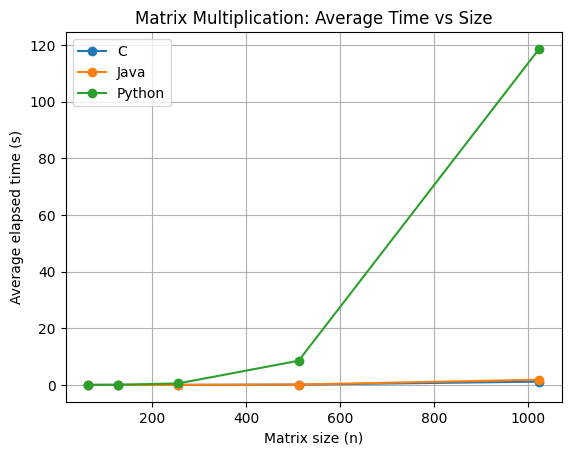
\includegraphics[width=.85\linewidth]{avg_time_by_language.png}
  \caption{Average elapsed time by language and matrix size (markers show means over runs).}
\end{figure}

\begin{figure}[H]
  \centering
  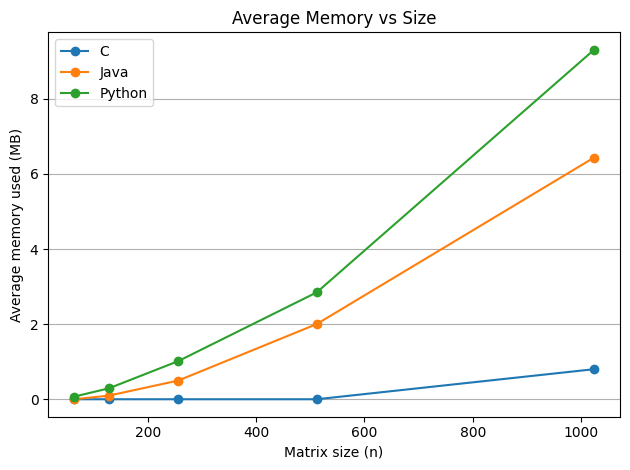
\includegraphics[width=.85\linewidth]{avg_memory_by_language.png}
  \caption{Average memory consumption by language and matrix size.}
\end{figure}

\begin{figure}[H]
  \centering
  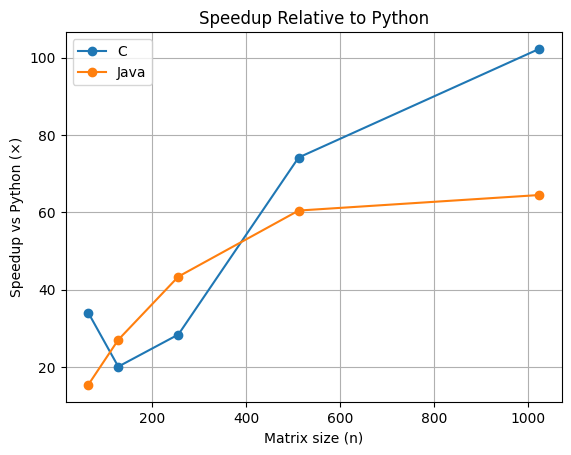
\includegraphics[width=.85\linewidth]{speedup_vs_python.png}
  \caption{Speedup relative to Python (higher is better).}
\end{figure}

% Auto-generated by plot_benchmarks.py
% Grouped bar charts and boxplot grids
\begin{figure}[H]
  \centering
  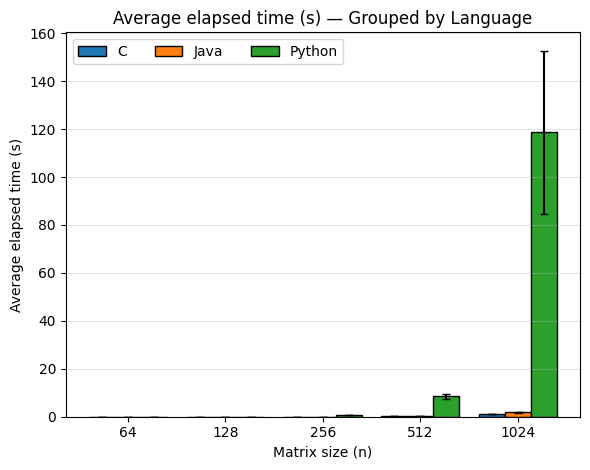
\includegraphics[width=.90\linewidth]{bar_time_grouped.png}
  \caption{Average elapsed time with standard-deviation error bars (grouped by language and matrix size).}
  \label{fig:bar-time}
\end{figure}

\begin{figure}[H]
  \centering
  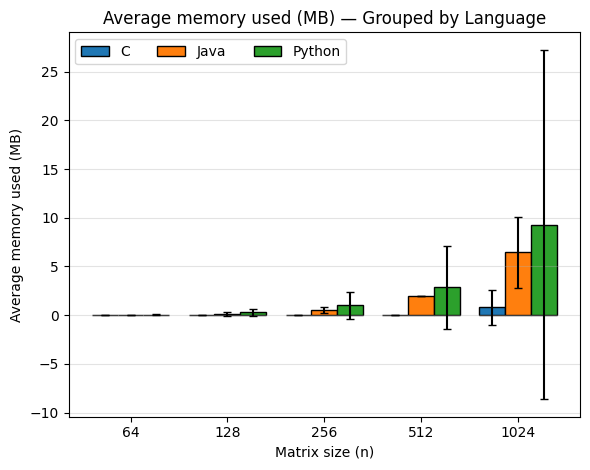
\includegraphics[width=.90\linewidth]{bar_mem_grouped.png}
  \caption{Average memory usage with standard-deviation error bars (grouped by language and matrix size).}
  \label{fig:bar-mem}
\end{figure}

\begin{figure}[H]
  \centering
  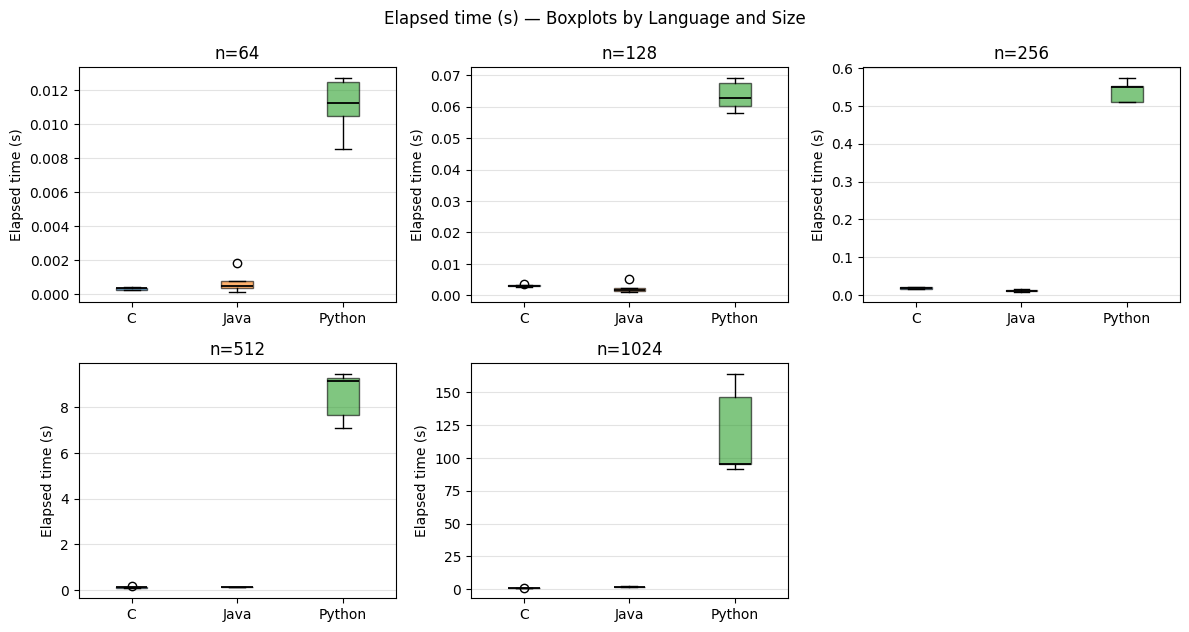
\includegraphics[width=.90\linewidth]{box_time_all_sizes.png}
  \caption{Elapsed time distributions (boxplots) by language across all matrix sizes.}
  \label{fig:box-time}
\end{figure}

\begin{figure}[H]
  \centering
  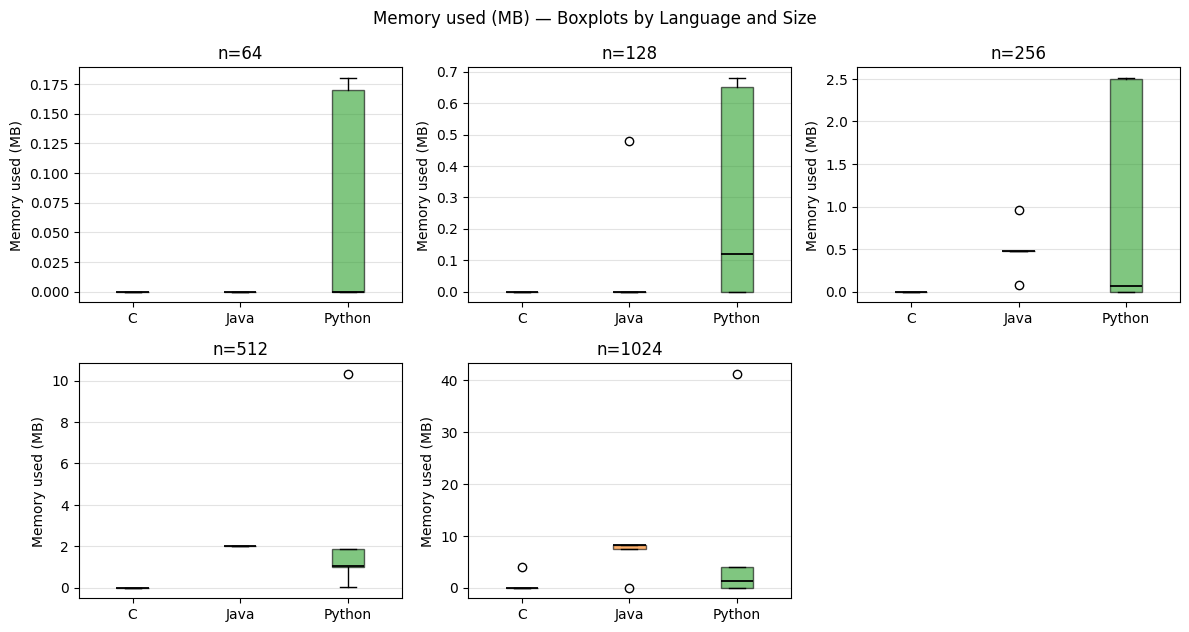
\includegraphics[width=.90\linewidth]{box_mem_all_sizes.png}
  \caption{Memory usage distributions (boxplots) by language across all matrix sizes.}
  \label{fig:box-mem}
\end{figure}


\begin{table}[H]
\centering
\caption{Per-language summary statistics (mean $\pm$ std).}
\label{tab:summary}
\begin{tabular}{lrrrrr}
\toprule
Language & Size & Runs & Avg time (s) & Avg mem (MB) & Note \\
\midrule
C & 64 & 5 & 0.000325 $\pm$ 0.000073 & 0.00 $\pm$ 0.00 & ~ \\
C & 128 & 5 & 0.003167 $\pm$ 0.000330 & 0.00 $\pm$ 0.00 & ~ \\
C & 256 & 5 & 0.018991 $\pm$ 0.003366 & 0.00 $\pm$ 0.00 & ~ \\
C & 512 & 5 & 0.115088 $\pm$ 0.020415 & 0.00 $\pm$ 0.00 & ~ \\
C & 1024 & 5 & 1.159879 $\pm$ 0.022769 & 0.80 $\pm$ 1.79 & ~ \\
Java & 64 & 5 & 0.000723 $\pm$ 0.000661 & 0.00 $\pm$ 0.00 & ~ \\
Java & 128 & 5 & 0.002353 $\pm$ 0.001642 & 0.10 $\pm$ 0.22 & ~ \\
Java & 256 & 5 & 0.012428 $\pm$ 0.003182 & 0.50 $\pm$ 0.32 & ~ \\
Java & 512 & 5 & 0.141220 $\pm$ 0.007584 & 2.00 $\pm$ 0.00 & ~ \\
Java & 1024 & 5 & 1.840129 $\pm$ 0.191275 & 6.43 $\pm$ 3.62 & ~ \\
Python & 64 & 5 & 0.011078 $\pm$ 0.001683 & 0.07 $\pm$ 0.10 & ~ \\
Python & 128 & 5 & 0.063536 $\pm$ 0.004740 & 0.29 $\pm$ 0.35 & ~ \\
Python & 256 & 5 & 0.538847 $\pm$ 0.028067 & 1.01 $\pm$ 1.36 & ~ \\
Python & 512 & 5 & 8.535703 $\pm$ 1.071202 & 2.85 $\pm$ 4.23 & ~ \\
Python & 1024 & 5 & 118.612292 $\pm$ 34.122409 & 9.30 $\pm$ 17.93 & ~ \\
\bottomrule
\end{tabular}
\end{table}
\section{Discussion}
As expected, C generally leads on raw runtime due to its ahead-of-time compilation and minimal runtime overhead. Java follows closely after just-in-time warm-up. Pure-Python triple loops are substantially slower, but with vectorized libraries (NumPy/BLAS) Python can achieve performance competitive with C---left for future work. The observed memory deltas are modest because input matrices are reused and only the output matrix is written.

\section{Threats to Validity}
(1) JIT warm-up effects in Java can skew the first run. (2) Background processes, turbo/thermal throttling, and power profiles affect timings. (3) Measurement of ``memory used'' differs slightly across platforms and APIs. We mitigate these threats by using multiple runs and reporting standard deviations.

\section{Conclusion}
The naive $O(n^3)$ kernel scales cubically across all languages. Results reflect language/runtime overhead rather than algorithmic differences. Future extensions include blocked/tiling variants, multithreaded versions, and BLAS-backed implementations to approach hardware limits.

\section*{Artifacts and Reproducibility}
\begin{itemize}
  \item GitHub repository: \url{https://github.com/seergiohrndz7/Individual-Assingment.git}.
  \item Unified CSV: \texttt{data/results.csv}.
\end{itemize}

\bibliographystyle{plain}
\bibliography{refs}
\end{document}
